
\section*{Overview}


This tutorial demonstrates how to accommodate variation in the substitution process across sites of an alignment.
In the preceding tutorials, we assumed that all sites in an alignment evolved under an identical substitution process.
This assumption is likely to be violated biologically, since different nucleotide sites are subject to different selection pressures, such as depending on which gene or codon position the site belongs to.
Here, we will demonstrate how to specify---and select among---alternative \emph{mixed models} using \RevBayes.
This is commonly referred to as partitioned-data analysis, where two or more subsets of sites in our alignment are assumed to evolve under distinct processes.

This tutorial will construct two multi-gene models.
The first model, PS0, assumes all genes evolve under the same process parameters.
The second model, PS1, assumes all genes evolve according to the same process, but each gene has it's own set of process parameters.
The third model, PS2, partitions the data not only by gene, but also by codon position.
Each analysis will generate a {\it maximum a posteriori} tree to summarize the inferred phylogeny.
An advanced exercise introduces how to compute Bayes factors to select across various partitioning schemes.

All of the files for this analysis are provided for you and you can run these without significant effort using the \cl{source()} function in the \RevBayes~console, e.g.
{\tt \begin{snugshade*}
\begin{lstlisting}
source("RevBayes_scripts/model_PS0.Rev")
\end{lstlisting}
\end{snugshade*}}

If everything loaded properly, then you should see the program begin running the Markov chain Monte Carlo analysis needed for estimating the posterior distribution. If you continue to let this run, then you will see it output the states of the Markov chain once the MCMC analysis begins.

\subsection*{Requirements}
We assume that you have previously completed the following tutorials:
\begin{itemize}
\item RB\_Getting\_Started
\item RB\_Data\_Tutorial
\item RB\_CTMC\_Tutorial
\item RB\_BayesFactor\_Tutorial
\end{itemize}
Accordingly, we will assume that you know how to execute and load data into \RevBayes, are familiar with some basic commands, and know how to perform Bayes factor comparisons to select among competing substitution models.



%%%%%%%%
%%   Data   %%
%%%%%%%%
\section*{Data and files}

We provide several data files that we will use in this tutorial; these are the same datasets that we have used in previous tutorials.
In the \cl{data} folder, you will find the following files
\begin{itemize}
\item
\cl{primates\_cytb.nex}: Alignment of the \textit{cytochrome b} subunit from 23 primates representing 14 of the 16 families (\textit{Indriidae} and \textit{Callitrichidae} are missing).
\item
\cl{primates\_cox2.nex}: Alignment of the \textit{COX-II} gene from the same 23 primates species.
\end{itemize}



\section*{Introduction}

Variation in the evolutionary process across the sites of nucleotide sequence alignments is well established, and is an increasingly pervasive feature of datasets composed of gene regions sampled from multiple loci and/or different genomes.
Inference of phylogeny from these data demands that we adequately model the underlying process heterogeneity; failure to do so can lead to biased estimates of phylogeny and other parameters \citep{Brown2007}.
%To accommodate process heterogeneity within and/or between various gene(omic) regions, we will evaluate the support for various partition schemes using Bayes factors to compare the marginal likelihoods of the candidate partition schemes.

Accounting for process heterogeneity involves adopting a `mixed-model' approach, \citep{Ronquist2003} in which the sequence alignment is first parsed into a number of partitions that are intended to capture plausible process heterogeneity within the data.
The determination of the partitioning scheme is guided by biological considerations regarding the dataset at hand.
For example, we might wish to evaluate possible variation in the evolutionary process within a single gene region (\EG between stem and loop regions of ribosomal sequences), or among gene regions in a concatenated alignment (\EG comprising multiple nuclear loci and/or gene regions sampled from different genomes).
The choice of partitioning scheme is up to the investigator and many possible partitions might be considered for a typical dataset.

%Next, a substitution model is specified for each predefined process partition (using a given model-selection criterion, such as Bayes factors).
In this exercise, we assume that each partition evolved under an independent general-time reversible model with gamma-distributed rates across sites (GTR+$\Gamma$). 
Under this model the observed data are conditionally dependent on the exchangeability rates ($\theta$), stationary base frequencies ($\pi$), and the degree of gamma-distributed among-site rate variation ($\alpha$), as well as the unrooted tree topology ($\Psi$) and branch lengths ($\nu$).
We show the graphical model representation of the GTR+$\Gamma$ mode in Figure \ref{pipeline}. 
When we assume different GTR+$\Gamma$ models for each partitions, this results in a composite model, in which all sites are assumed to share a common, unrooted tree topology and proportional branch lengths, but subsets of sites (`data partitions') are assumed to have independent substitution model parameters.
This composite model is referred to as a \emph{mixed model}. 
%\taha{need to change the graphical model above to have the same symbols as in this paragraph since this refers to the figure \ref{pipeline} and it may be harder to change that figure.}



Finally, we perform a separate MCMC simulation to approximate the joint posterior probability density of the phylogeny and other parameters.  Note that, in this approach, the mixed model is a fixed assumption of the inference (\IE the parameter estimates are conditioned on the specified mixed model), and the parameters for each process partition are independently estimated.

For most sequence alignments, several (possibly many) partition schemes of varying complexity are plausible {\it a priori}, which therefore requires a way to objectively identify the partition scheme that balances estimation bias and error variance associated with under- and over-parameterized mixed models, respectively.
Increasingly, mixed-model selection is based on \textit{Bayes factors} \citep[{\it e.g.},][]{Suchard2001}, which involves first calculating the marginal likelihood under each candidate partition scheme and then comparing the ratio of the marginal likelihoods for the set of candidate partition schemes \citep{Brandley2005,Nylander2004,Mcguire2007}.
The analysis pipeline that we will use in this tutorial is depicted in Figure \ref{pipeline}.

\begin{figure}[ht!]
\centering
\fbox{\includegraphics[width=6.8in,angle=0]{\ResourcePath figures/pipeline.eps}}
\caption{\small The analysis pipeline for Exercise 1. We will explore three partition schemes for the primates dataset.
The first model (the `uniform model', $M_0$) assumes that all sites evolved under a common GTR+$\Gamma$ substitution model.
The second model (the `moderately partitioned' model, $M_1$) invokes two data partitions corresponding to the two gene regions (cytB and cox2), and assumes each subset of sites evolved under an independent GTR+$\Gamma$ model.
The final mixed model (the `highly partitioned' model, $M_2$) invokes four data partitions---the first two partitions corresponds to the cytB gene region, where the first and second codon position sites share a partition distinct from the third codon position sites, and the cox2 has two partitions of its own, partitioned by codon positions in the same way---and each data partition is assumed evolved under an independent GTR+$\Gamma$ substitution model.
Note that we assume that all sites share a common tree topology, $\Psi$, and branch-length proportions, $\nu$, for each of the candidate partition schemes.
We perform two separate sets of analyses for each mixed model---a Metropolis-coupled MCMC simulation to approximate the joint posterior probability density of the mixed-model parameters, and a `stepping-stone' MCMC simulation to approximate the marginal likelihood for each mixed model.
The resulting marginal-likelihood estimates are then evaluated using Bayes factors to assess the fit of the data to the three candidate mixed models.  
}
\label{pipeline}
\end{figure}
\newpage


